\documentclass{article}
\usepackage[margin=1in]{geometry}
\usepackage{graphicx}

\graphicspath{{./screenshots/}}
\usepackage{xeCJK}
\usepackage{lipsum}
\setCJKmainfont{Noto Serif CJK TC}

\author{Andr\'es Ponce (0616110) \
\and
彭思安}
\title{Network Systems Capstone Lab 2 Report}

\renewcommand{\familydefault}{\sfdefault}
\begin{document}
\maketitle
\section{Part 1}
\subsection{After you complete Steps 1--1}
\subsubsection{Can h2 ping h3? Briefly explain why or why not.}
At the first step, each router has their static IP address configured.
However, there are yet no rules as to how to send a packet from one subnet
to another.
Since these two hosts are on the same subnet, similar to Lab 1 we can use the 
ARP protocol with Ethernet to send data. 
This only relies on the IP and MAC address of the hosts, which is independent 
from the routing tables in the router.

\subsubsection{Can h2 ping h4? Briefly explain why or why not.}
When a packet reaches r1, there is still no routing information for how to get to 
r4 to deliver the packet.
At the beginning, none of the routers know exactly how to route the packages
or what interface to use and what address should receive thte packet.

Thus, whenever we attempt to send the packet each router will not have a specified
routing behavior.
\subsection{Complete \texttt{topology.py} so that all hosts, except h1, can ping one 
another. Take a screenshot to show that your topology is correct.}
Once we set the IP addresses of the routers for each of their interfaces, and add
the routing connections with the \texttt{route add -net \dots}command, our routers
know which interface should receive the incoming packets.

\begin{figure}[h]
		\centering
		\label{fig:topo}
		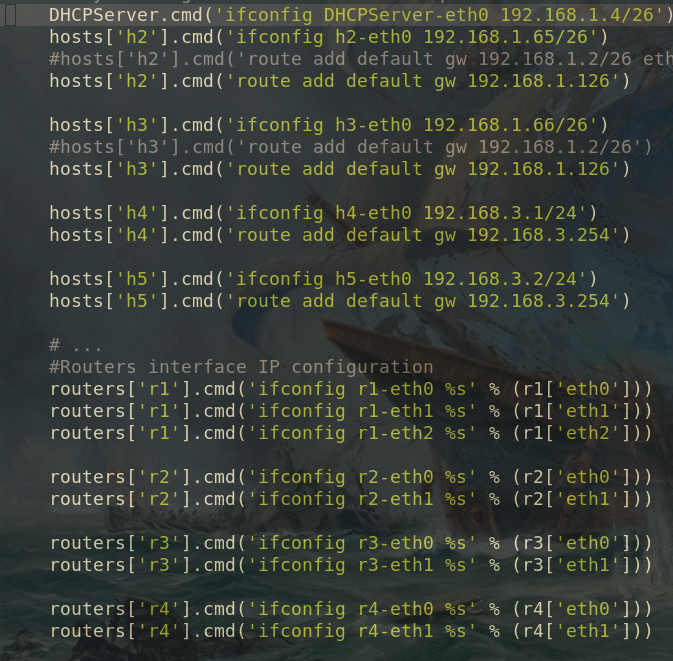
\includegraphics[scale=0.3]{topoConf.png}
		\caption{Output of the network after setting routing tables.}
\end{figure}

In Fig~\ref{fig:topo}, the ping commands can successfully
link all the hosts in the network, and only h1 remains isolated.
\section{Part2}
\subsection{Capture DHCP messages and show the IPs and MACs}
\begin{figure}[h]
	\centering
	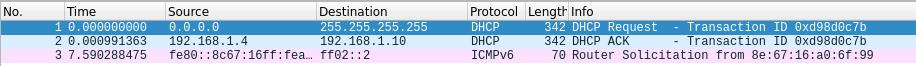
\includegraphics[scale=0.3]{h1dhcp.png}
	\caption{The messges sent from h1-eth0 when we attempt a DHCP request.}
\end{figure}
\subsection{Can hosts other than h1 acquire IP addresses from the DHCP server? 
Briefly explain your answer.}
No, if we attempt to do \texttt{h5 dhclient h5-eth0}, the IP address of the host 
will remain the same, and this happens for all the remaining hosts.
They already have a defined IP address, so connecting to a DHCP will not result
in any new address.
Also, the DHCP server is located in another local network.
\subsection{What does r1 do on the packets from h1 to h5, and h5 to h1,
respectively? Capture packets to explain your answer.}
To see the effects of passing through a router, we can run the \texttt{h1 ping h5}
command.
\begin{figure}
		\centering
		\label{fig:r1-eth1}
		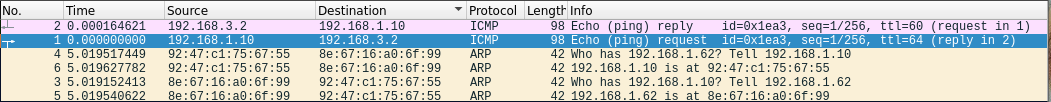
\includegraphics[scale=0.5]{r1eth-1.png}
		\caption{Capturing the packets on \textbf{r1-eth1}.}
\end{figure}
In \ref{fig:r1-eth1}, we are sending the packet to our default gateway with our 
destination set to \texttt{h5}'s address.

\begin{figure}[h]
		\centering
		\label{fig:r1-eth0}
		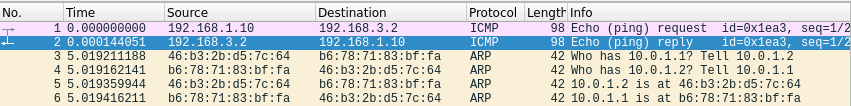
\includegraphics[scale=0.5]{r1-eth0.png}
		\caption{Capturing the packets on \textbf{r1-eth0}.}
\end{figure}

In \ref{fig:r1-eth0}, we see the router r1 asking for the address of the other
routers on the way to h5.
However, the router will be the one in charge of sending the packet rather than
the host.
So h1 is only responsible for getting the packet to the router.

\section{Part 3}
\subsection{Capture all ICMP messages received y h1 and explain why h1 can only derive only
1st, 2nd, and 5th hop details.}
\begin{figure}[h]
		\centering
		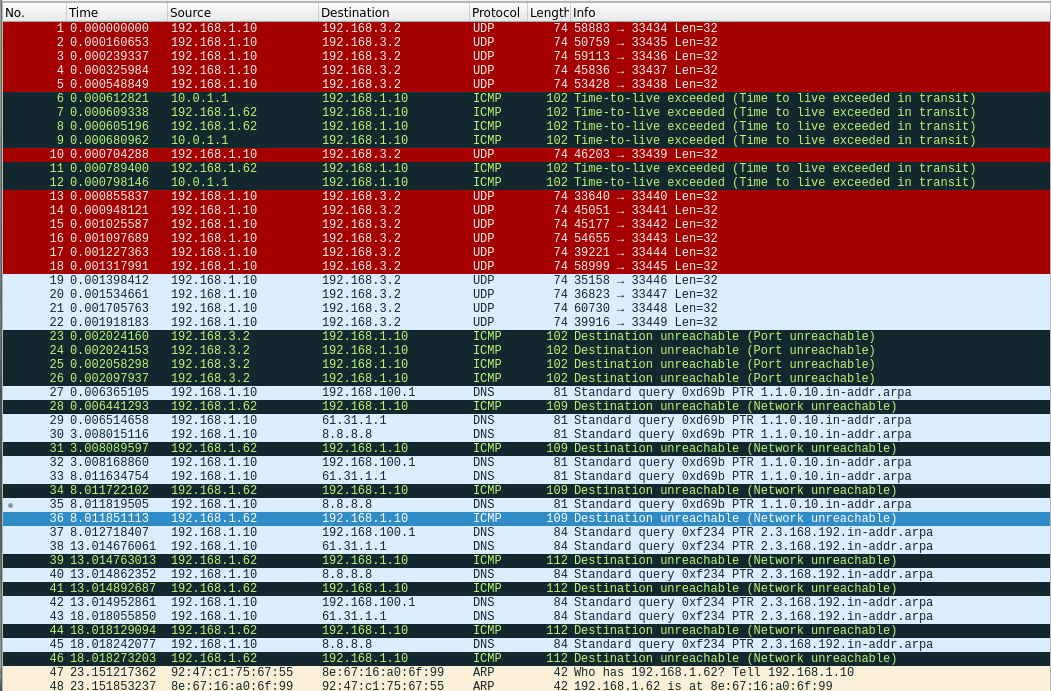
\includegraphics[scale=0.3]{traceroute.png}
		\caption{All the messages needed to trace a path from h1 to h5.}
\end{figure}
H1 can only receive the first and second hops due to the fact that the router
is going to send the packet using its own IP address, which is why we cannot see
any of the packets from the middle of the route.

We can also see the messges from the fifth hop, because on the fifth hop, 
h5 is responding directly to h1. 
When the return packets go through the router, the router will again replace h1's 
address in the destination.
That's why we can see the packet sent from h5 to h1, but not r4 to r1. 
\subsection{H1 uses some ICMP messages to derive 1st and 2nd hop details.
What are the type(s) and sender(s) of the ICMP messages?}
Traceroute works by incrementally increasing the TTL of each packet. 
When the TTL is exceeded, the router will respond to h1 with an ICMP TTL exceeded
message.
Then h1 will know to increase this value.

\subsection{H1 uses some ICMP messages to derive 5th
What are the type(s) and sender(s) of the ICMP messages?}
In this case, the sender is h5, and the message is a Destination Unreachable ICMP message.
\end{document}
